\section{Avstörningsmetoder}

\subsection{Allmänt}
För att prova ut ett filter, som bäst löser ett visst
radiostörningsproblem, kan man behöva tillgång till ett
filtersortiment

Som exempel nämns bl.a. filter i SSA:s avstörningslådor.

\subsection{Nätfilter}
\textbf{
HAREC a.\ref{HAREC.a.9.3.1.1}\label{myHAREC.a.9.3.1.1}
}

Nätledningar kan fungera som antenn. I sändarfallet kan HF-signaler
komma ut i elnätet genom nätledningen och störa andra apparater både
genom direktanslutning och strålning. I mottagarfallet kan HF-signaler
uppfångas av nätledningen, ledas in i apparaterna och LF-detekteras
där. För att förhindra sådana störningar behövs ett nätfilter.

Nätfiltret skall vara dimensionerat för den nätström, som apparaten är
avsäkrad för och bör anslutas så nära apparaten som möjligt.  Om
filtret inte kan placeras där, kan det vara nödvändigt att även skärma
nätledningen mellan filtret och apparaten och jorda skärmen.

\begin{wrapfigure}{R}{0.5\textwidth}
  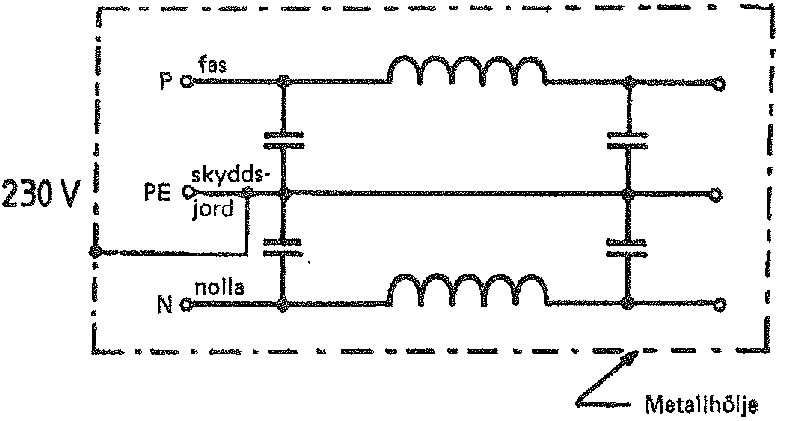
\includegraphics[width=0.5\textwidth]{images/bild_2_9-01}
  \caption{Nätfilter}
  \label{fig:bildII9-1}
\end{wrapfigure}

Om ledningen förses med t.ex. en serieinduktans - en drossel - så
dämpas HF-signalerna. En drossel kan man göra t.ex.  genom att linda
upp några varv av nätsladden närmast apparaten på toroider eller en
eller flera sammanlagda ferritstavar. I svåra fall kan det behövas ett
bredbandigt nätfilter, liknande det på bild \ref{fig:bildII9-1}.

Det kan förekomma kraftiga spänningstransienter (spänningsstötar) på
belysningsnätet. Dessa transienter kan leda till felfunktioner i
anslutna apparater. För att förebygga sådana fel kan man koppla in ett
överspänningsfilter, som kan vara separat eller sammanbyggt med
nätfiltret

\subsection{Lågpassfilter}

\begin{figure}
  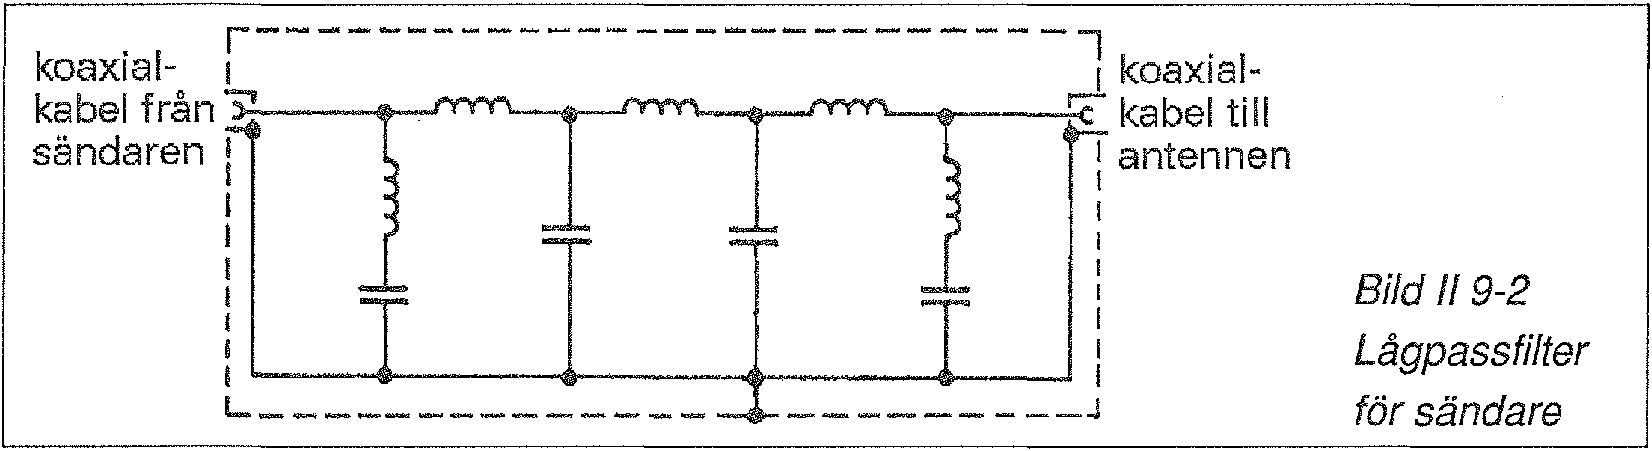
\includegraphics[width=\textwidth]{images/bild_2_9-02}
  \caption{Lågpassfilter för sändare}
  \label{fig:bildII9-2}
\end{figure}

Lågpassfilter släpper igenom signaler med frekvenser under filtrets
gränsfrekvens.

Ett lågpassfilter med lämpligt vald gränsfrekvens dämpar
t.ex. övertonsutstrålningen från en sändare, vars sändarfrekvens
ligger under filtrets gränsfrekvens medan övertonerna ligger över dess
gränsfrekvens.

Övertoner kan dämpas med lågpassfilter. En överton är i detta
sammanhanhang en multipel av sändningsfrekvensen (grundtonen)
exempelvis för 3.5 MHz grundtonen = (1:a harmoniska) 3.5 MHz, 1:a
överton = (2:a harmoniska) 7.0 MHz, 2:a överton = (3:e harmoniska)
10.5 MHz o.s.v.

Viktigt för avsedd filterverkan är, att filtret ansluts med korrekt
impedansanpassning och med kortast möjliga ledningar. Detta gäller
f.ö. alla filter.

Utstrålning utanför sändningsslagets tillåtna bandbredd anses som
``icke önskad utstrålning''. Vidare gäller att sådan utstrålning från
amatörradiosändare skall hållas så låg som dagens amatörradioteknik
medger.  Bild \ref{fig:bildII9-2} visar principen för lågpassfiltret TP 30 för
kortvåg, med gränsfrekvensen 36 MHz, att kopplas mellan sändaren och
antennledningen. Med denna gränsfrekvens dämpas övertoner från sändare
så att risken för TV-störningar minskar.

\subsection{Högpassfilter}

Högpassfilter släpper igenom signaler med frekvenser över filtrets
gränsfrekvens.

\begin{figure}
  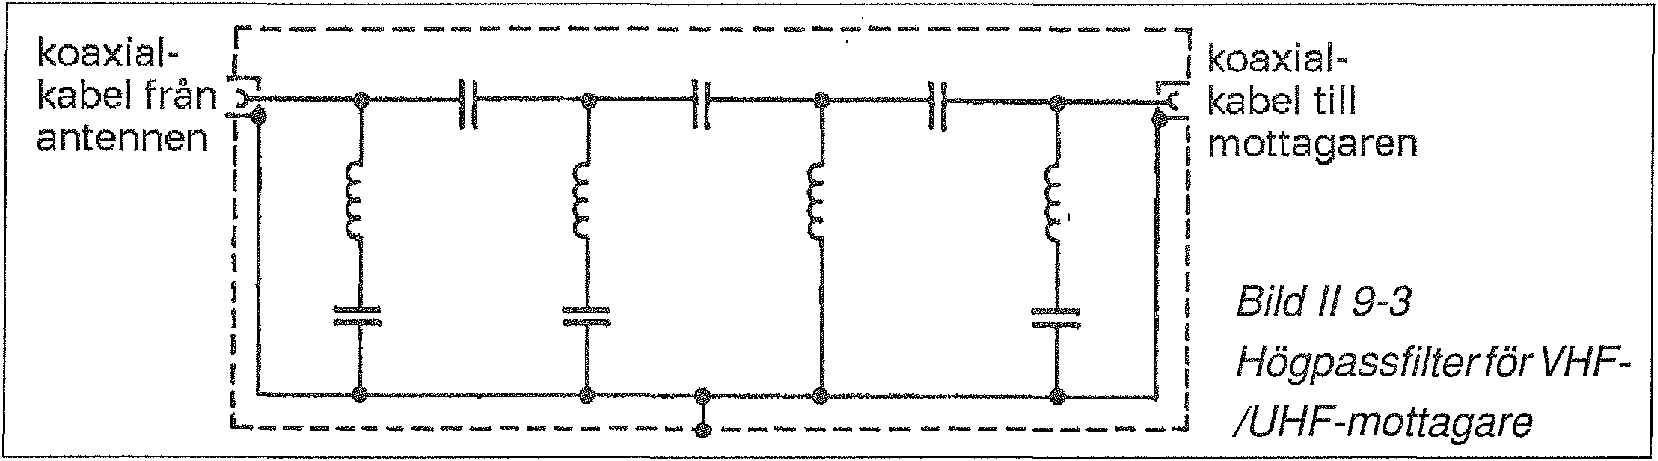
\includegraphics[width=\textwidth]{images/bild_2_9-03}
  \caption{Högpassfilter för VHF/UHF-mottagare}
  \label{fig:bildII9-3}
\end{figure}

Bild \ref{fig:bildII9-3} visar principen för högpassfiltret HP 40-S med
gränsfrekvensen 47 MHz, att kopplas in mellan antennledningen och en
mottagare för VHF eller högre frekvenser.

Störningar kommer inte alltid ``utifrån''.  De kan t.ex. alstras i
bredbandiga antennförstärkare, vilka lätt överstyrs av alla slags
signaler från ett stort frekvensområde. Man kan då koppla in ett
högpassfilter före bredbandsförstärkaren, men en bättre lösning är att
byta till en väl skärmad passbands- eller ännu hellre
kanalförstärkare.

Koaxialkablar med täta skärmar och rätt monterade anslutningskontakter
är också viktigt för en lyckad avstörning.

\subsection{Spärrfilter och sugkretsar}

\begin{figure}
  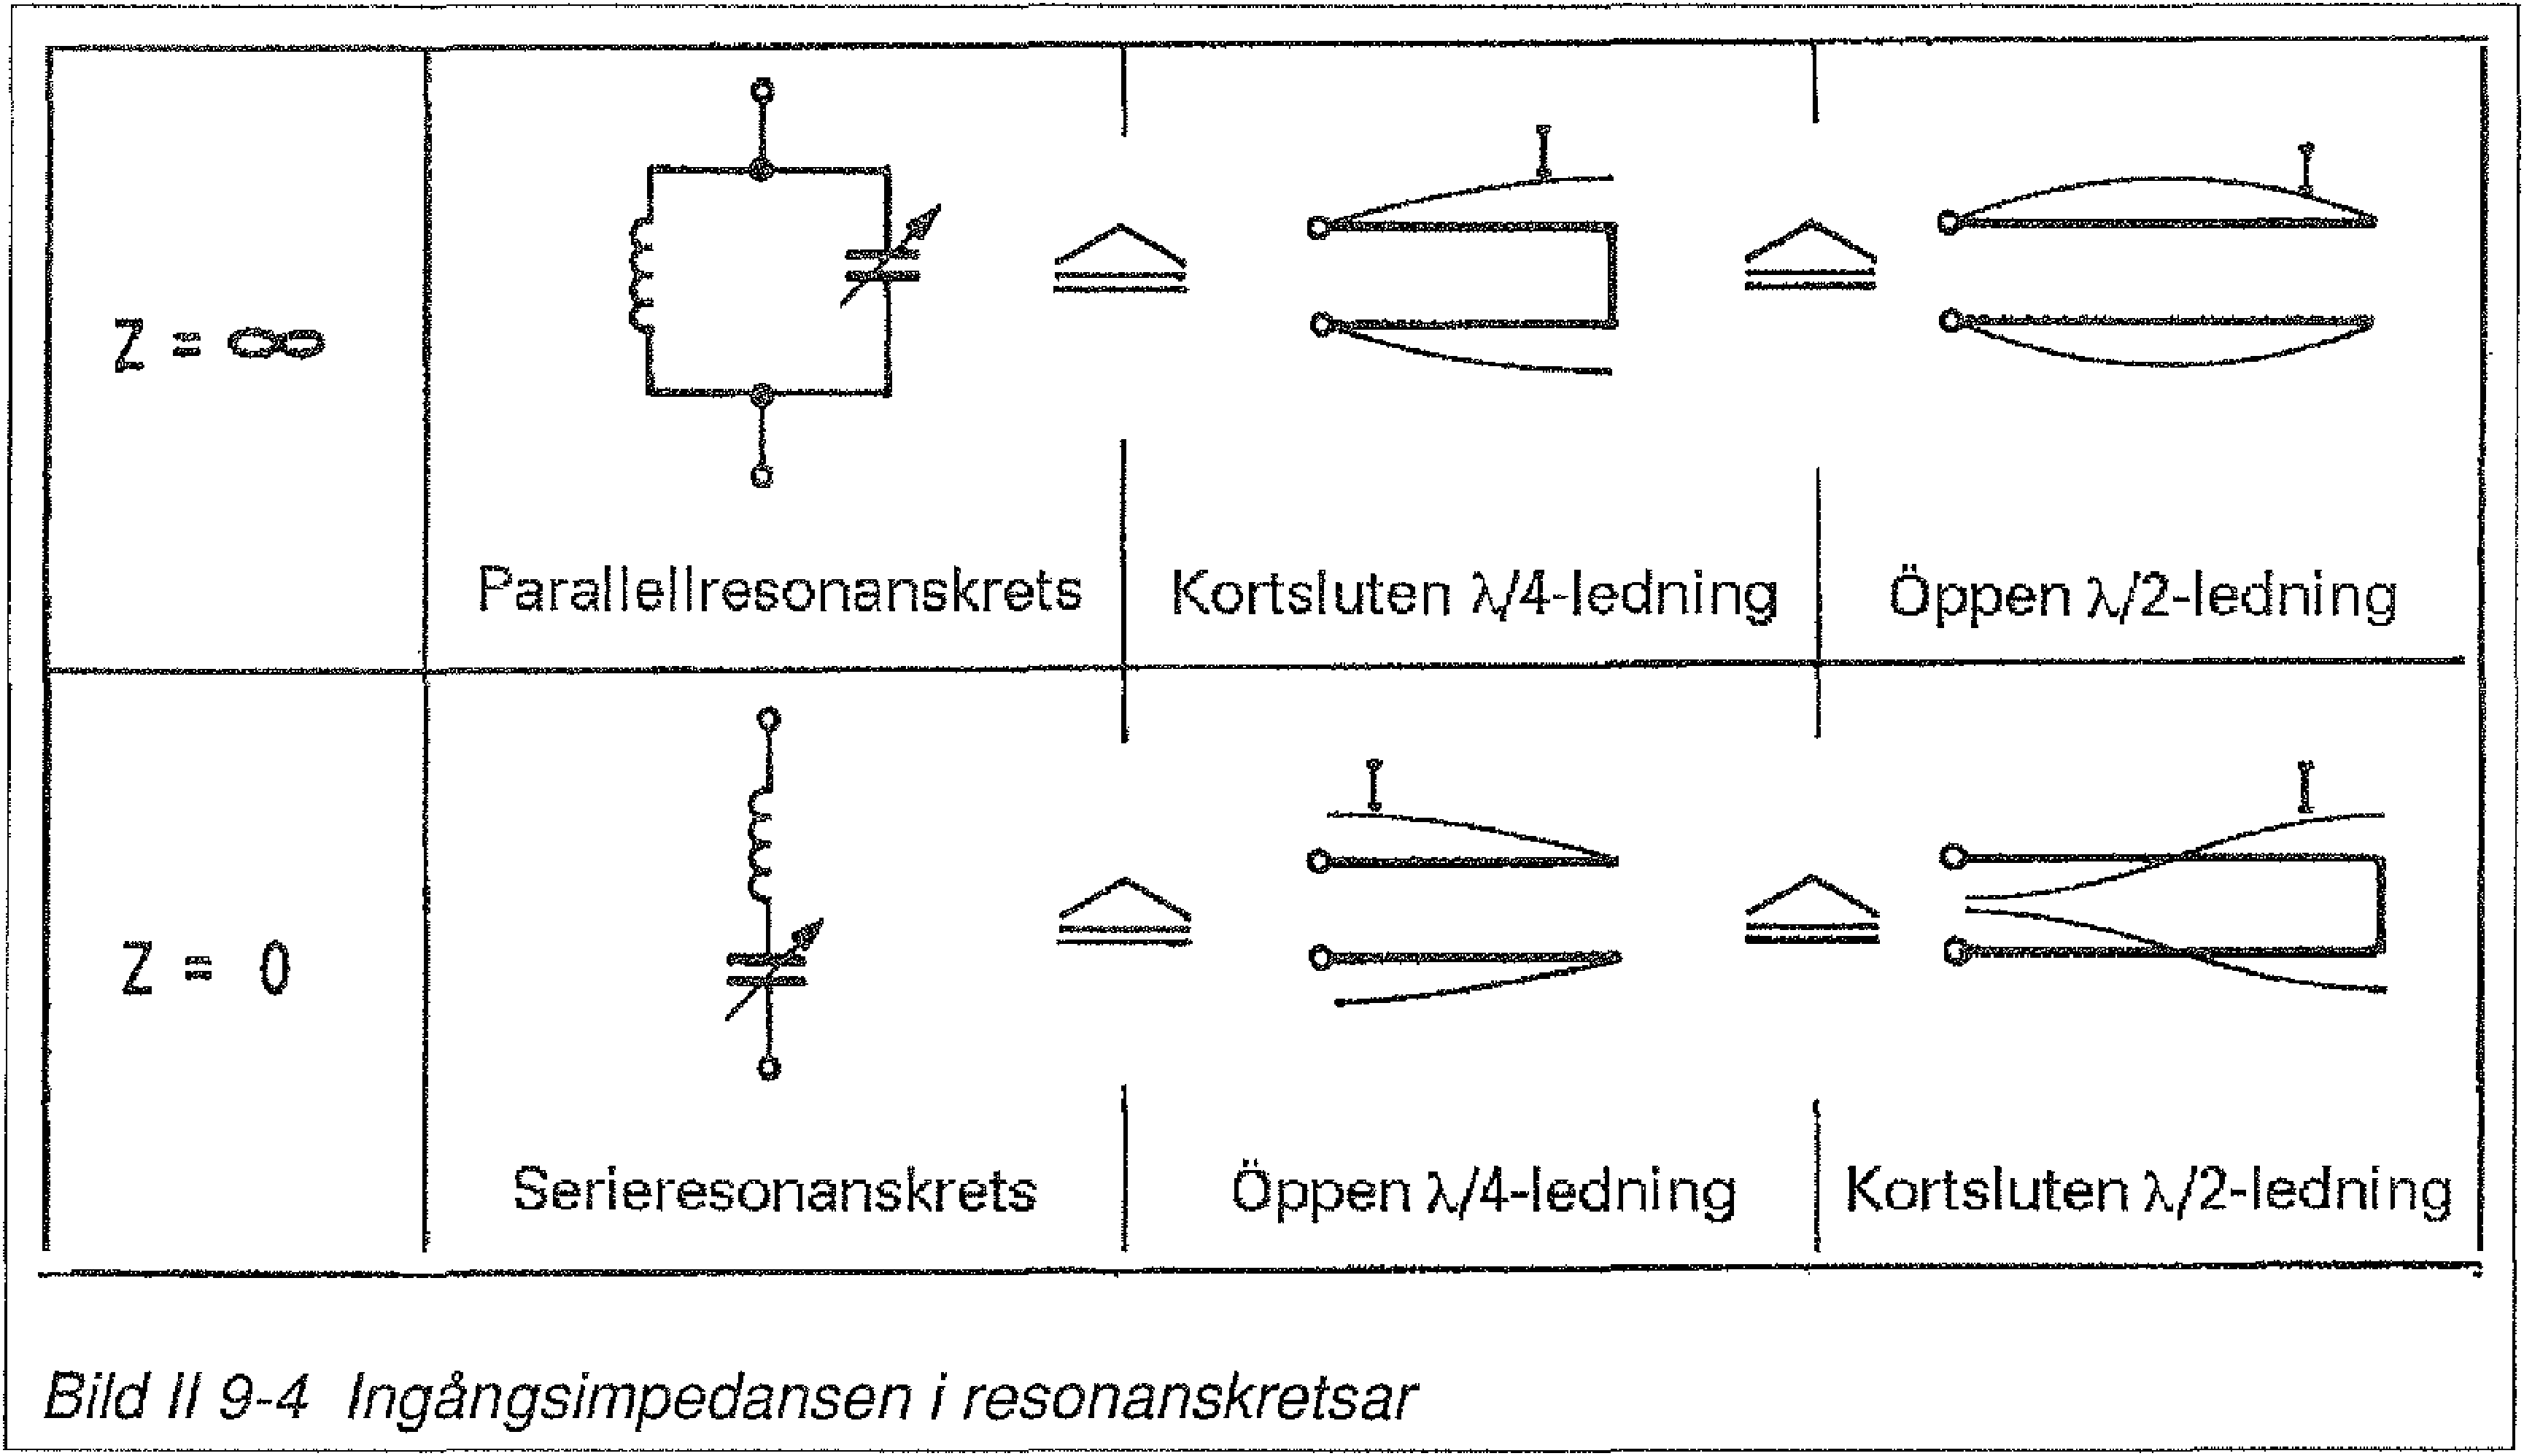
\includegraphics[width=\textwidth]{images/bild_2_9-04}
  \caption{Ingångsimpedansen i resonanskretsar}
  \label{fig:bildII9-4}
\end{figure}

\begin{figure}
  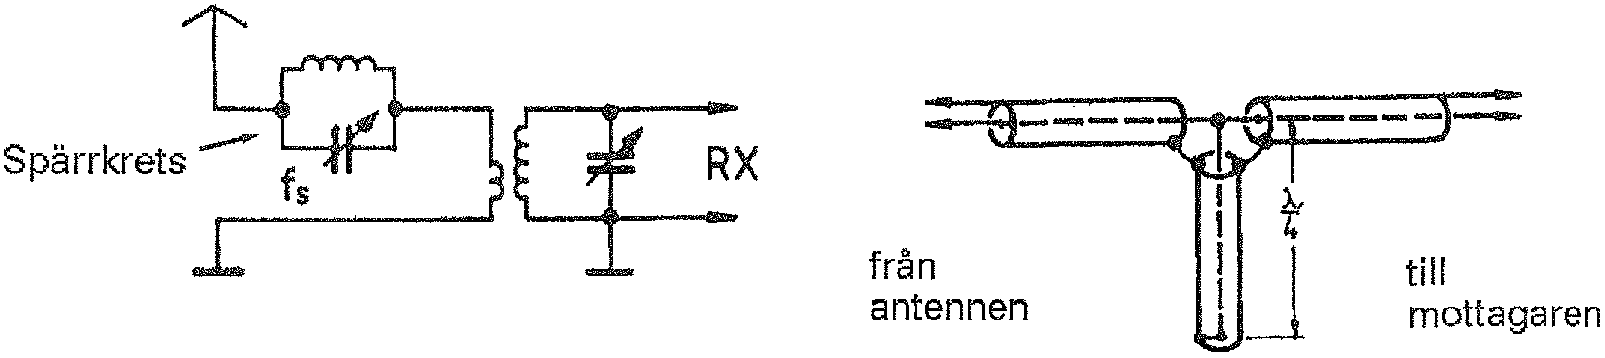
\includegraphics[width=\textwidth]{images/bild_2_9-05}
  \caption{Spärrfilter för mottagare}
  \label{fig:bildII9-5}
\end{figure}

\begin{figure}
  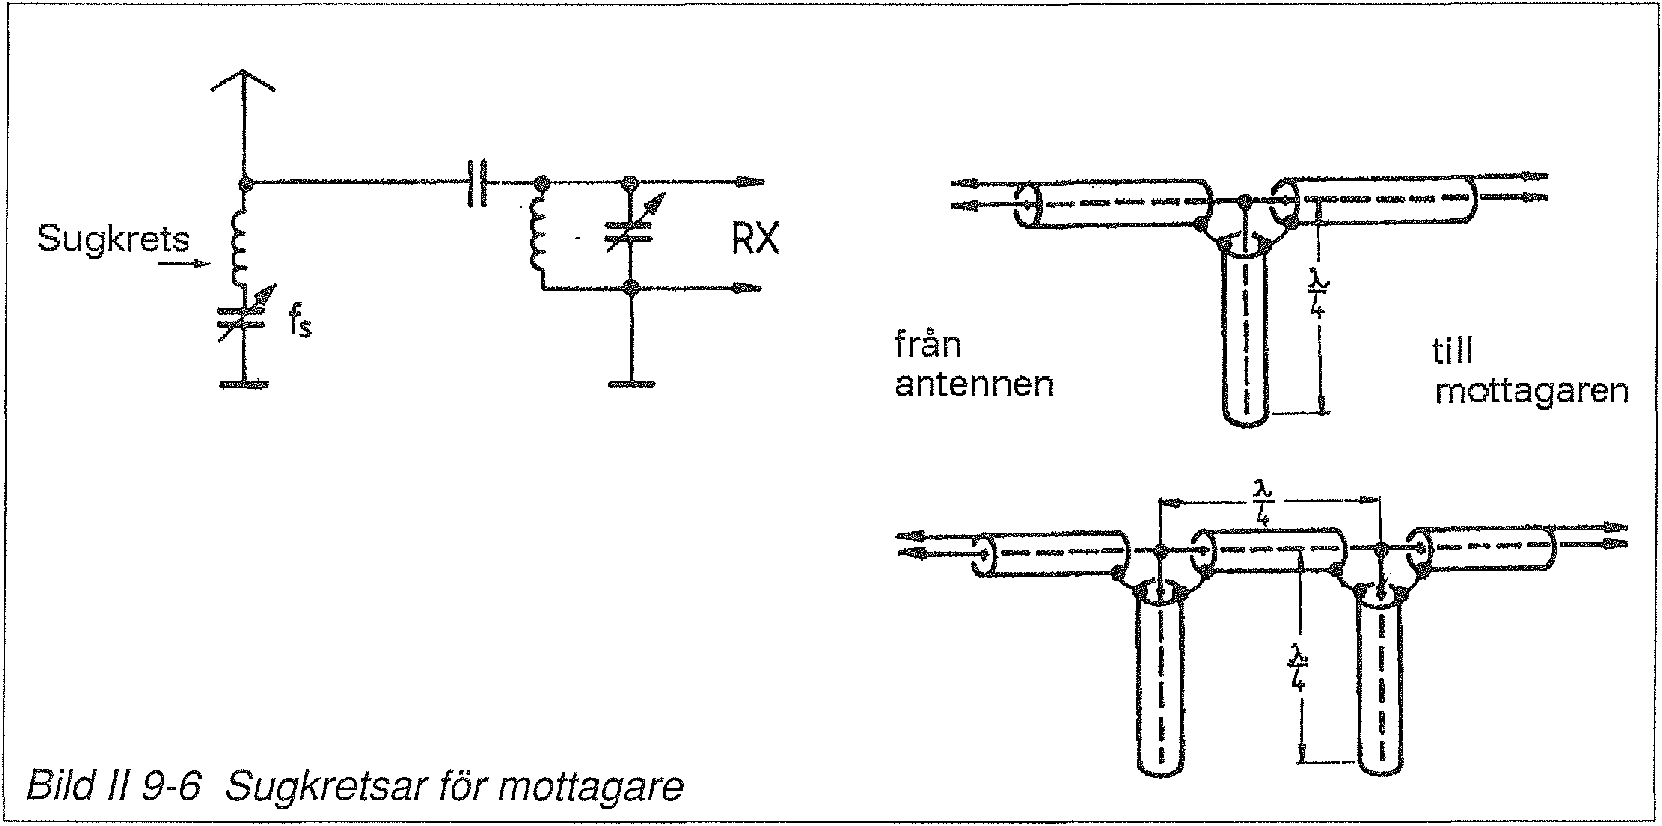
\includegraphics[width=\textwidth]{images/bild_2_9-06}
  \caption{Sugkretsar för mottagare}
  \label{fig:bildII9-6}
\end{figure}

Om en störande signal råkar finnas inom passbandet för mottagaren kan
man undertrycka - ``spärra'' - den signalen med ett spärr- eller
sugfilter. Vilket man väljer är inte kritiskt.

Den störande signalen kan ``spärras'' med en parallellresonanskrets i
serie med mottagaringången (Bild \ref{fig:bildII9-5}). Kretsen består av en induktans
och en kapacitans.

Om man använder en stub som resonanskrets - t.ex. en koaxialkabel - så
skall den ha längden \(\lambda/4\) och vara ``kortsluten'' eller ha
längden \(\lambda/2\) och vara ``öppen''.

Man kan även kortsluta - ``suga bort'' den störande signalen med en
serieresonanskrets parallellt över mottagaringången (Bild \ref{fig:bildII9-6}). Om
man då använder en stub, så skall den ha längden \(\lambda/4\) och
vara ``öppen'' eller ha längden \(\lambda/2\) och vara ``kortsluten''.

Den störande signalen kan undertryckas ytterligare med fler stubar,
som ordnas som i Bild \ref{fig:bildII9-6}. Filtret består då av öppna
\(\lambda/4\)-stubar, som utgör avgreningar från antennkabeln med ett
avstånd av \(\lambda/4\).

(Om stubarna i detta filter kortsluts, så bildas ett bandpassfilter i
stället).

Exempel på kommersiella spärrfilter är SF~145-S för 144 MHz och
SF~435-S, för 435 MHz amatörband. De är avsedda att kopplas in före
mottagare som störs av amatörradiosändningar.

SF 145-S spärrar amatörbandet 144 - 148 MHz och släpper igenom banden
0 - 120 och 174 - 870 MHz.

SF 435-S spärrar amatörbandet 430 - 440 MHz och släpper igenom 0 -
350 och 470 - 870 MHz.

\subsection{Nät- och skärmströmfilter för mottagning}

\begin{wrapfigure}[14]{R}{0.5\textwidth}
  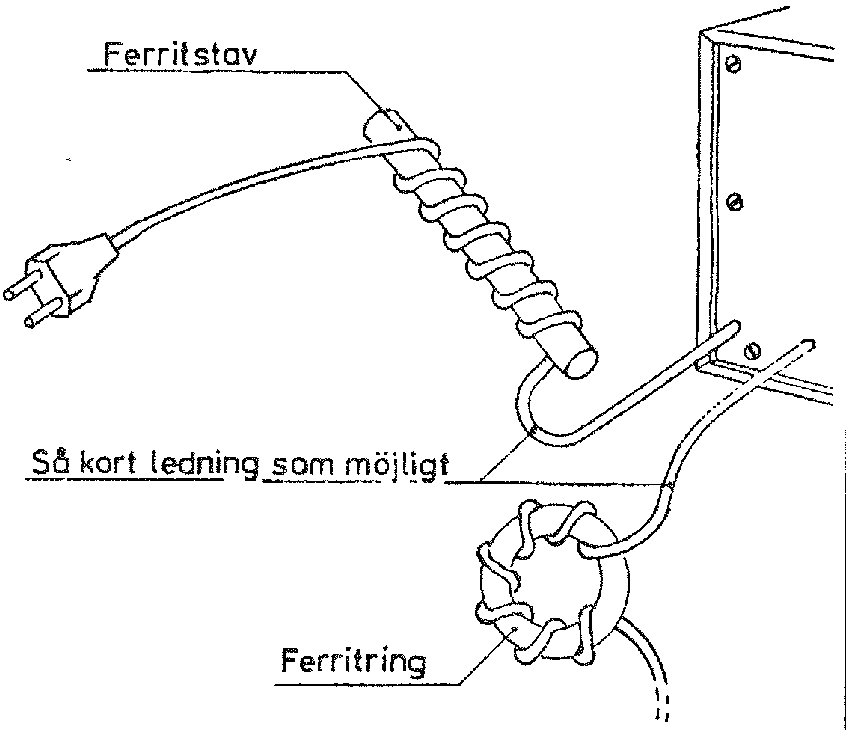
\includegraphics[width=0.5\textwidth]{images/bild_2_9-07}
  \caption{Nät- och skärmströmfilter}
  \label{fig:bildII9-7}
\end{wrapfigure}

Bild \ref{fig:bildII9-7}

\begin{rev-omarbetas}
Utsidan av antennkabelns skärm kan också fungera som antenn. Särskilt
i skärmskarvar kan HF-strömmar läcka ut och in. De kan då passera förbi
eventuella antennförstärkare, filter etc. och orsaka störningar.

I enkla fall kan yttre skärmströmmar stoppas med att linda upp kabeln
några varv på ferritstavar eller genom en stor ferritring som på
bilden. En nätkabel, s.k. sladdställ, får inte kapas och skarvas.

\hilight{TODO: Prata om common mode-strömmar här}
\end{rev-omarbetas}

\subsection{Phono-ingångsfilter (TBA~302)}

\begin{wrapfigure}[18]{R}{0.5\textwidth}
  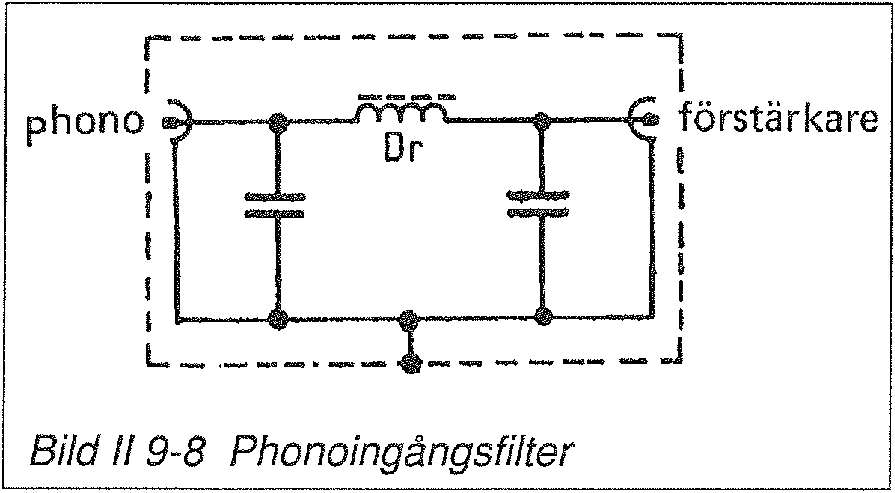
\includegraphics[width=0.5\textwidth]{images/bild_2_9-08}
  \caption{Phonoingångsfilter}
  \label{fig:bildII9-8}
%\end{wrapfigure}
%\begin{wrapfigure}{R}{0.5\textwidth}
  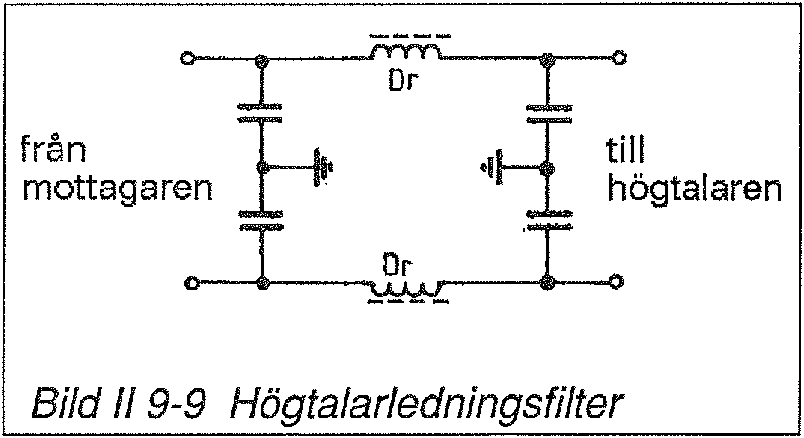
\includegraphics[width=0.5\textwidth]{images/bild_2_9-09}
  \caption{Högtalarledningsfilter}
  \label{fig:bildII9-9}
\end{wrapfigure}

Bild \ref{fig:bildII9-8}

Störande påverkan från radiosändningar kan uppstå om
anslutningsledningarna till phono-ingången i LF-förstärkare är dåligt
skärmade och avkopplade. Sådana störningar kan avhjälpas med ett
filter.

\subsection{Högtalarledningsfilter (EM 502-B)}

Bild \ref{fig:bildII9-9}

HF-instrålning på högtalarledningar kan ha en störande påverkan. Detta
kan undvikas genom koppla in HF-drosslar i ledningarna.  Dessa
drosslar bör vara skärmade så att de inte verkar som antenner
istället.

I enklare fall kan det räcka med att byta till skärmade högtalarkablar
eller att linda upp en sträcka av ledningarna på en ferritkärna.

\subsection{Avkoppling av HF-signaler}
\textbf{
HAREC a.\ref{HAREC.a.9.3.1.2}\label{myHAREC.a.9.3.1.2}
}

\begin{figure}
  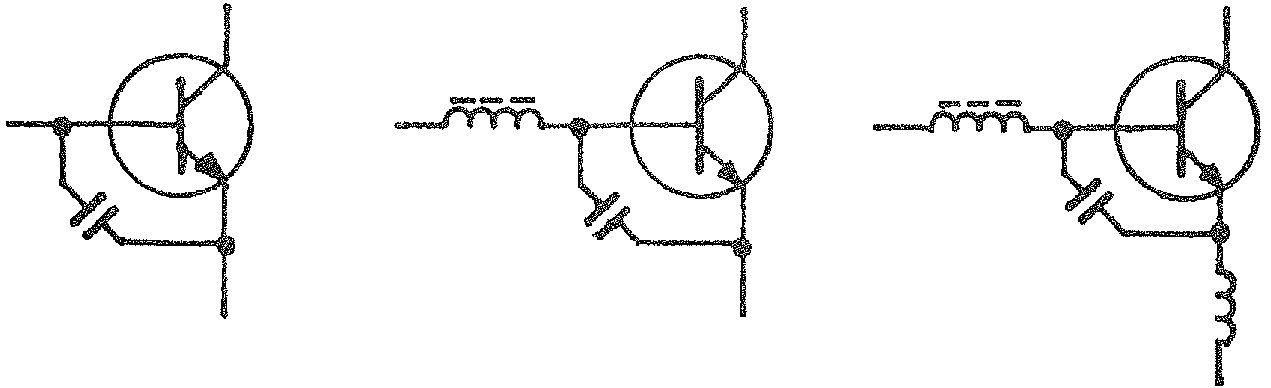
\includegraphics[width=\textwidth]{images/bild_2_9-10b}
  \caption{HF-avkopplad bas på tre sätt}
  \label{fig:bildII9-10b}
\end{figure}

\begin{wrapfigure}[19]{R}{0.5\textwidth}
  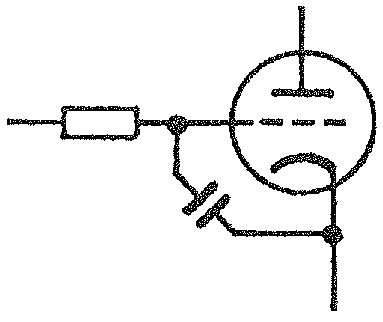
\includegraphics[width=0.5\textwidth]{images/bild_2_9-10a}
  \caption{HF-avkopplat styrgaller}
  \label{fig:bildII9-10a}

  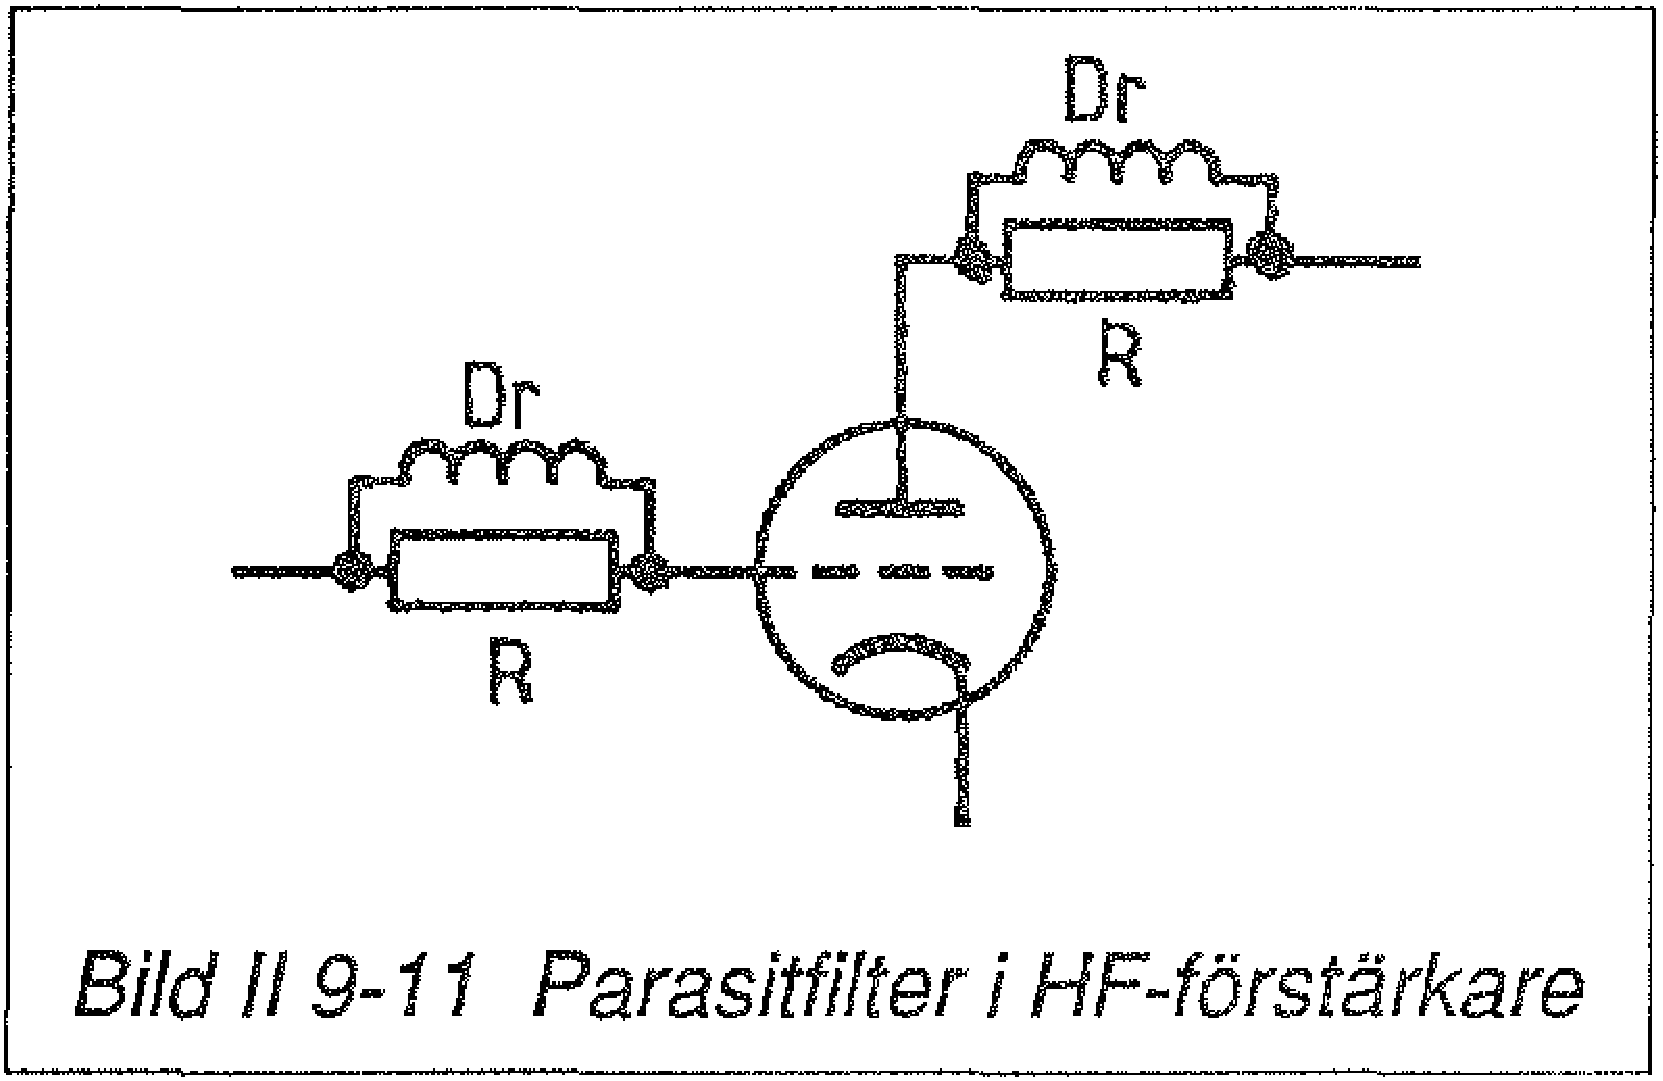
\includegraphics[width=0.5\textwidth]{images/bild_2_9-11}
  \caption{Parasitfilter i HF-förstärkare}
  \label{fig:bildII9-11}
\end{wrapfigure}

Med avkoppling av en signal menas att den avleds från en signalväg
till en annan. Vid avstörning avkopplas vanligen den störande
signalen till systemjord.

Störimmuniteten i mottagare kan alltså förbättras genom att LF-ingång-
arna HF-avkopplas med kondensatorer och/eller HF-spärras med drosslar.

I svåra störningsfall kan det också bli nödvändigt med HF-avskärmning
av LF-ingångsstegen, liksom med ytterligare avstörningsfilter inne i
förstärkaren.

Sådana åtgärder innebär emellertid att konstruktionsändringar har
gjorts. Apparatens elsäkerhetsmärkningar är då ogiltiga.

Bild \ref{fig:bildII9-10a} och \ref{fig:bildII9-10b} visar några sätt att avkoppla en oönskad signal från
styrgallret i ett elektronrör respektive från basen i en transistor.

\subsection{Parasitfilter}

Bild \ref{fig:bildII9-11}

Förstärkarsteg kan råka i självsvängning, ofta på frekvenser i
VHF/UHF-området. Ett sätt att stoppa det är med s.k. parasitfilter.

\subsection{Nycklingsfilter}

Bild \ref{fig:bildII9-12}

När en bärvåg nycklas, så bildas övertoner.  Blandningsprodukter av
övertonerna och bärvågen hörs som knäppar på omkringliggande
frekvenser. Märk att övertoner uppstår vid all bärvågsnyckling - inte
bara vid morsetelegrafering!

När övergångstiden är kort (hård nyckling), så bildas fler övertoner
än när den är längre (mjuk nyckling). Knäpparna kan till en del dämpas
med ett nycklingsfilter där dels insvängningsförloppet bromsas med en
drossel i serie med nycklingskontakten och dels ursvängningsförloppet
med en seriekrets av en resister och en kondensator, kopplade
parallellt över nycklingskontakten.

\begin{wrapfigure}{R}{0.5\textwidth}
  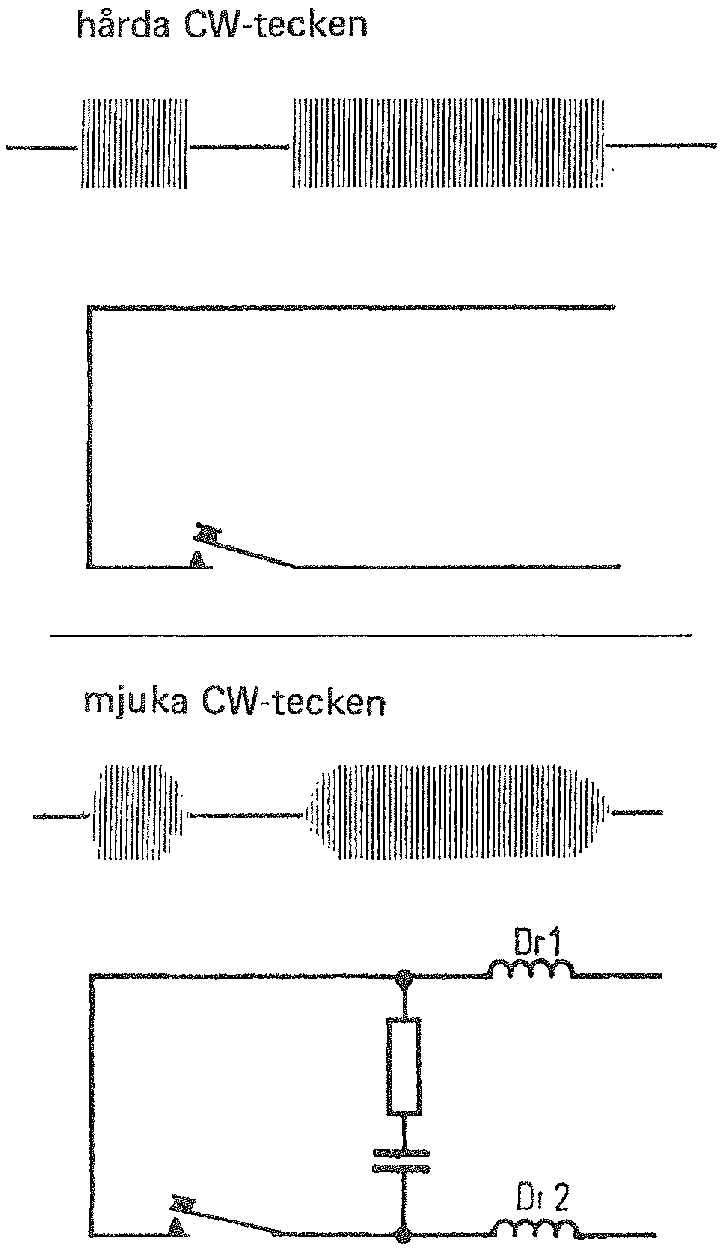
\includegraphics[width=0.5\textwidth]{images/bild_2_9-12}
  \caption{Nycklingsfilter}
  \label{fig:bildII9-12}
\end{wrapfigure}

\subsection{Förbättrad skärmning}
\textbf{
HAREC a.\ref{HAREC.a.9.3.1.3}\label{myHAREC.a.9.3.1.3}
}

HF-energi kan i olyckliga fall även stråla ut genom sändarens hölje
och in genom andra apparaters hölje. Det medför att apparaternas
skärmningar och jordning måste förbättras. Följ då
elsäkerhetsbestämmelserna!  Se även kapitel \ref{elektriskafält},
\ref{elektromagnetiskafält} och \ref{jordning}.
